%\newpage
\section{Final state interactions with spectator nucleons}
\mbox{}\vspace{-\baselineskip}
\label{sec:fsi}

Let's again consider the case when the exclusive reaction happens off a proton that is contained within a nucleus. The final hadrons, once produced, can then experience interactions with spectator nucleons. Meanwhile, spectator nucleons are extrinsic to the original exclusive reaction, and therefore any interaction with them breaks the energy-momentum conservation imposed on the reaction particles. As a consequence, final state interactions (FSI) with spectator nucleons introduce disturbances to the distributions of missing quantities.


In this Section, the influence of such interactions on distributions of considered missing quantities is traced. This task, however, is complicated by 
the fact that no methods to properly simulate FSI effects currently exist due to their complex nature. 


\everypar{\looseness=-1}
Therefore, in this Section, a naive modeling of FSI with spectator nucleons is attempted. The basic idea that underlies this modeling is that all mechanisms that possibly can happen during FSI have one simple feature in common; namely, they alter the momentum of the participating hadrons. 
This feature may be used to track manifestations of FSI effects kinematically. The modeling is hence of kinematic character, as it fully focuses on hadron momentum alterations and disregards particular mechanisms behind these alterations.



To perform such a modeling, one can assume that the final hadrons of the considered exclusive reaction experience momentum alterations as in the case of FSI with spectator nucleons\footnote[5]{In general this modeling suits for any kind of momentum alterations that break the energy-momentum conservation between the reaction particles.}. For simplicity, the following assumptions can be introduced, (i) only one registered final hadron is affected, (ii) the type of the affected hadron is the same among all affected events, and (iii) only the magnitude of the hadron momentum changes\footnote[6]{The adequacy of the latter assumption may vary depending on the type of the affected hadron, the type (gain/loss) and degree of momentum alterations, and the underlying interaction mechanism.}.


Then for each event, the alterations of the hadron momentum can be parameterized by $p'_{h} = \varepsilon p_{h}$, where $p_{h}$ and $p'_{h}$ are the momentum magnitudes of the hadron before and after the alteration, respectively, and $\varepsilon >0$ reflects the alteration degree. One should also keep in mind that the variable $\varepsilon$ may have some distribution among events in the sample, and hence it is convenient to introduce here $\xi(\varepsilon)$ as the corresponding probability density function, which will come into play later in this Section.


\everypar{\looseness=-1}
Now, in order to trace the influence of FSI with spectator nucleons on the missing quantities $M_{X[0]}^{2}$ and $M_{X[\pi^{-}]}^{2}$, one can estimate these quantities for events affected by the aforementioned momentum alterations, i.e. for those events with $\varepsilon \neq $1. The quantity $M_{X[0]}^{2}$ can be expressed by\vspace{-0.69em}
\begin{equation}
\begin{aligned}
&M_{X[0]}^{2}&=&~(P^{\mu}_{h} -P'^{\mu}_{h})^{2} = [P^{\mu}_{h}]^{2} +\left [P'^{\mu}_{h}\right ]^{2}-2[P_{h}]_{\mu} P'^{\mu}_{h} \\
&&=&~2m^{2}_{h}-2 \left (E_{h}E'_{h} - (\overrightarrow{p}_{h}\cdot \overrightarrow{p}'_{h}) \right )\\
&&=&~2m^{2}_{h} - 2\left (\sqrt{m^{2}_{h}+p^{2}_{h}}\sqrt{m^{2}_{h}+\varepsilon^{2}p^{2}_{h}}-\varepsilon p^{2}_{h}\right ),\\[-7pt]
\end{aligned}\label{eq:mm0_fsi}
\end{equation}
where $m_{h}$ is the mass of the hadron that undergoes the momentum change.


\newpage

The final expression in Eq.~\eqref{eq:mm0_fsi} is always less than zero, regardless of both the value of $\varepsilon$ and hadron kinematics, as the comparison below demonstrates\footnote[7]{In this comparison the lower indices are dropped and the wedge symbol ($\wedge$) means ``compare~with".}.
\vspace{-0.3em}
\begin{equation}
\begin{aligned}
2m^{2} - 2(\sqrt{m^{2}+p^{2}}\sqrt{m^{2}+\varepsilon^{2}p^{2}}-\varepsilon p^{2})& ~~\wedge~~ 0&\\
m^{2} - \sqrt{m^{2}+p^{2}}\sqrt{m^{2}+\varepsilon^{2}p^{2}} +\varepsilon p^{2} &~~\wedge~~ 0&\\
m^{2}+\varepsilon p^{2} &~~\wedge~~ \sqrt{m^{2}+p^{2}}\sqrt{m^{2}+\varepsilon^{2}p^{2}}&\\
m^{4}+\varepsilon^{2}p^{4}+2m^{2}\varepsilon p^{2} &~~\wedge~~ m^{4} + p^{2}m^{2} + m^{2}\varepsilon^{2}p^{2}+\varepsilon^{2}p^{4}&\\
2m^{2}\varepsilon p^{2} &~~\wedge~~ p^{2}m^{2}+  m^{2}\varepsilon^{2}p^{2}&\\
0 &~~\wedge~~ p^{2}m^{2}(\varepsilon^{2}-2\varepsilon+1)&\\
0&~~<~~ p^{2}m^{2}(\varepsilon-1)^{2}&\\[-8pt]
\end{aligned}\label{eq:comp}
\end{equation}
%\vspace{-0.3em}
The quantity $M_{X[\pi^{-}]}^{2}$ in turn can be written as\vspace{-0.35em}
\begin{equation}
\begin{aligned}
&M_{X[\pi^{-}]}^{2}&=&~(P^{\mu}_{\pi^{-}}+ P^{\mu}_{h} -P'^{\mu}_{h})^{2} \\
&&=&~[P^{\mu}_{\pi^{-}}]^{2} +(P^{\mu}_{h} -P'^{\mu}_{h})^{2}+2\left [P_{\pi^{-}}\right ]_{\mu} \left (P^{\mu}_{h} -P'^{\mu}_{h}\right ) \\
&&=&~m_{\pi^{-}}^{2} + M_{X[0]}^{2} +2\left \{E_{\pi^{-}}(E_{h}-E'_{h}) - \overrightarrow{p}_{\pi^{-}}\cdot(\overrightarrow{p}_{h} - \overrightarrow{p}'_{h})\right \}\\
&&=&~m_{\pi^{-}}^{2} + M_{X[0]}^{2} +2\left \{(\overrightarrow{p}_{\pi^{-}}\cdot \overrightarrow{p}_{h})(\varepsilon-1) - E_{\pi^{-}}(E'_{h}-E_{h})\right \}.\\[-7pt]
\end{aligned}\label{eq:mm_pim_fsi}
\end{equation}



The final expression in Eq.~\eqref{eq:mm_pim_fsi} can be either greater or smaller than $m_{\pi^{-}}^{2}$ depending on the interrelation between the value of $M_{X[0]}^{2}$ (which is always negative) and the quantity in the curly brackets (which can have either sign).


\everypar{\looseness=-1}
As follows from Eqs.~\ref{eq:mm0_fsi} and ~\ref{eq:mm_pim_fsi}, the resulting shape of the missing mass distributions is determined by (i) the value of $\varepsilon$ and its distribution among the events in the sample, or in other words, on the probability density function $\xi(\varepsilon)$, (ii) the type of affected final hadron, and (iii) the reaction kinematics. The examples given below are intended to demonstrate the interplay of these factors. These examples test several types of the probability density function $\xi(\varepsilon)$ and consider separately two types of affected hadrons, i.e. proton and positive pion.


%\afterpage{\clearpage}
%\vspace{-0.5em}
\subsection{Illustrating examples}

\vspace{-0.325em}

First, in order to estimate the sensitivity of the missing quantities to hadron momentum alterations, it is convenient to consider the case when the value of $\varepsilon$ is fixed and different from one for all events in the sample. Under this assumption one can examine the distributions of the missing quantities for different fixed values of $\varepsilon$ considering separately the two types of affected final hadrons (the positive pion and the proton).




\afterpage{\clearpage}
\begin{figure}[htp]
\begin{center}
\framebox{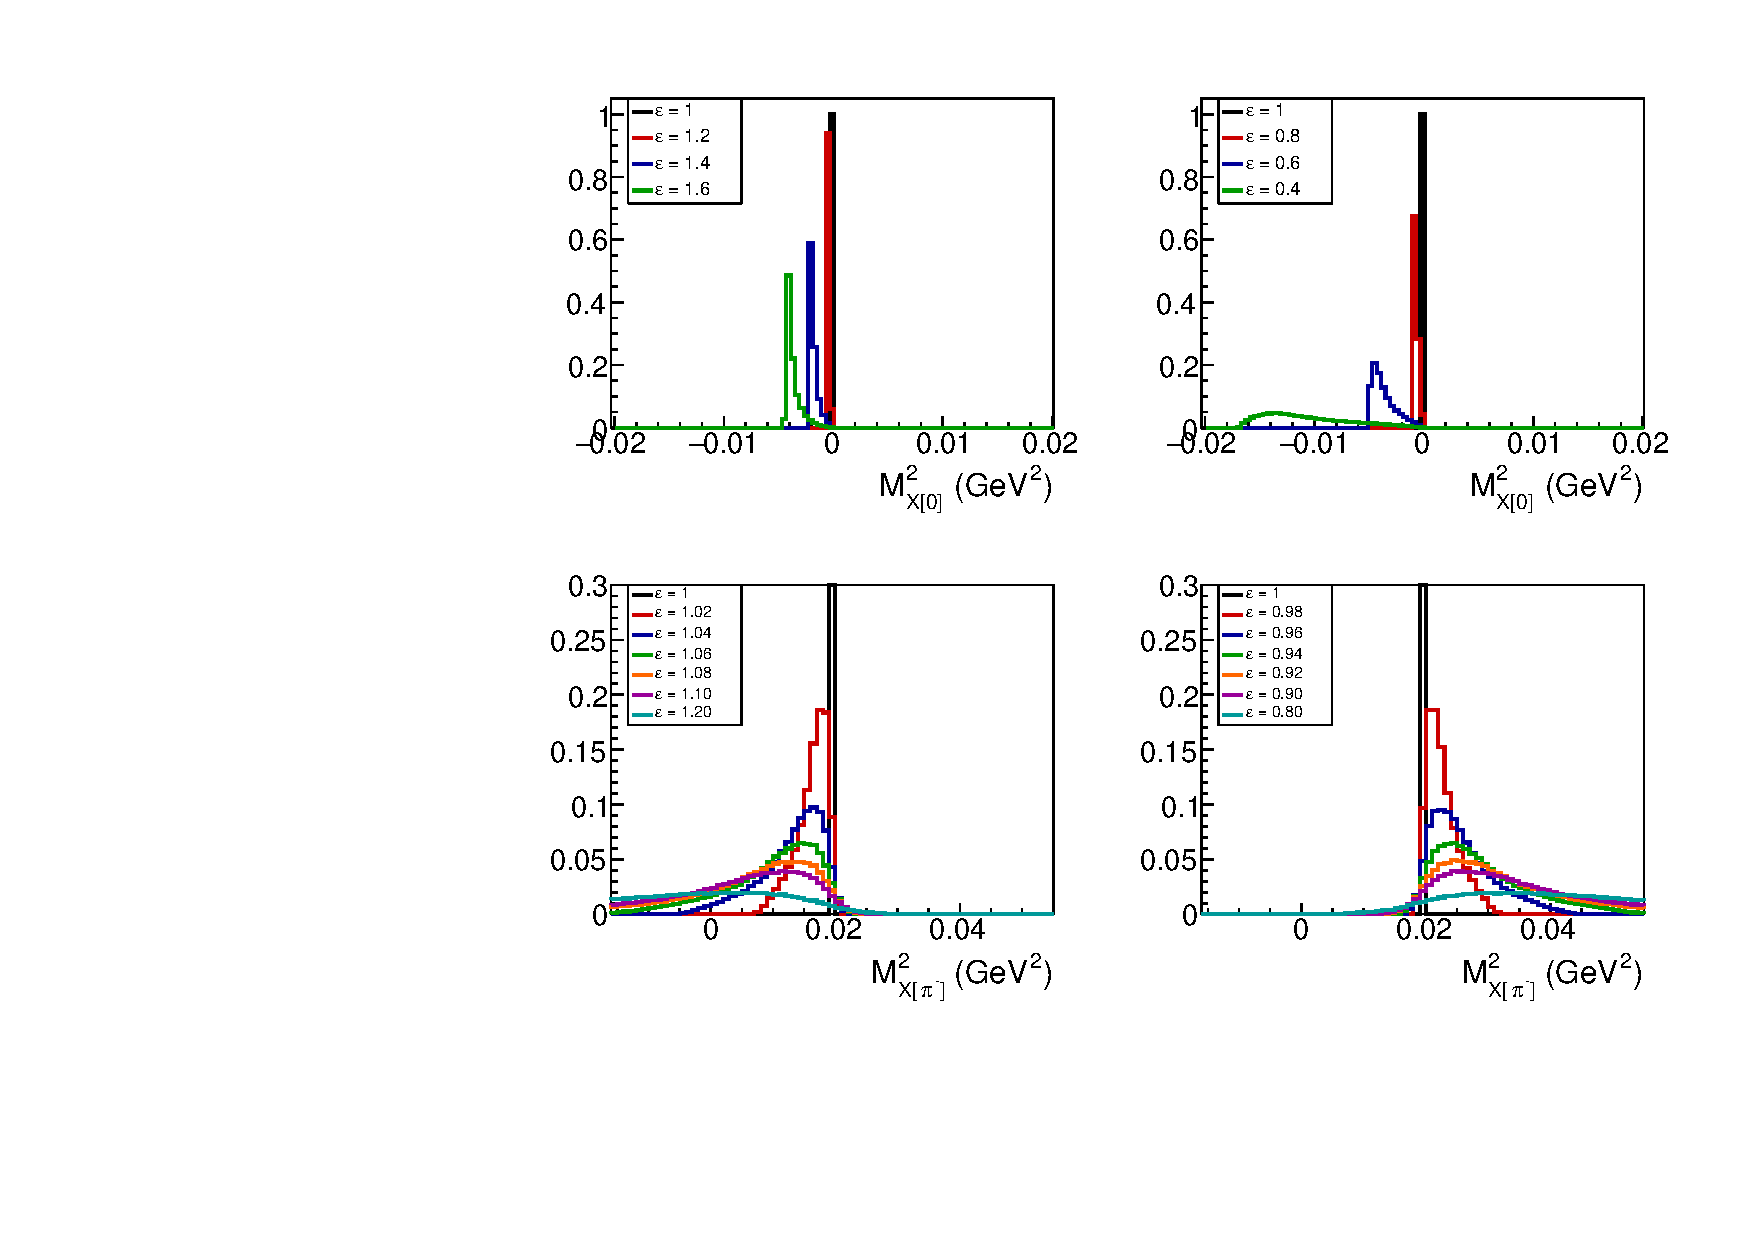
\includegraphics[width=\textwidth]{pictures/mm_pip_fsi_new2.pdf}}
\caption{\small Multi-colored histograms show the distributions of $M_{X[0]}^{2}$ (upper panels) and $M_{X[\pi^{-}]}^{2}$ (lower panels) plotted assuming that the $\pi^{+}$ momentum magnitude changes as $p'_{\pi^{+}} = \varepsilon p_{\pi^{+}}$ for all events in the sample. Different colors correspond to different values of $\varepsilon$. Black histograms are given as a reference and correspond to the case when no momentum alterations happen (i.e. $\varepsilon = 1$ for all events). All shown histograms contain equal numbers of events and are normalized in a way that the maximum of the $\varepsilon=1$  histogram is equal to one. The histograms that correspond to the same missing quantity have identical binning. For the quantity $M_{X[\pi^{-}]}^{2}$, shown in the lower panels, note the following, (i) the distributions are zoomed in on small $y$ and (ii) the change in $\varepsilon$ values between the magenta and cyan histograms is five times larger than for all other neighboring histograms. } \label{fig:mm_pip_fsi}
\end{center}
\end{figure}

\begin{figure}[htp]
\begin{center}
\framebox{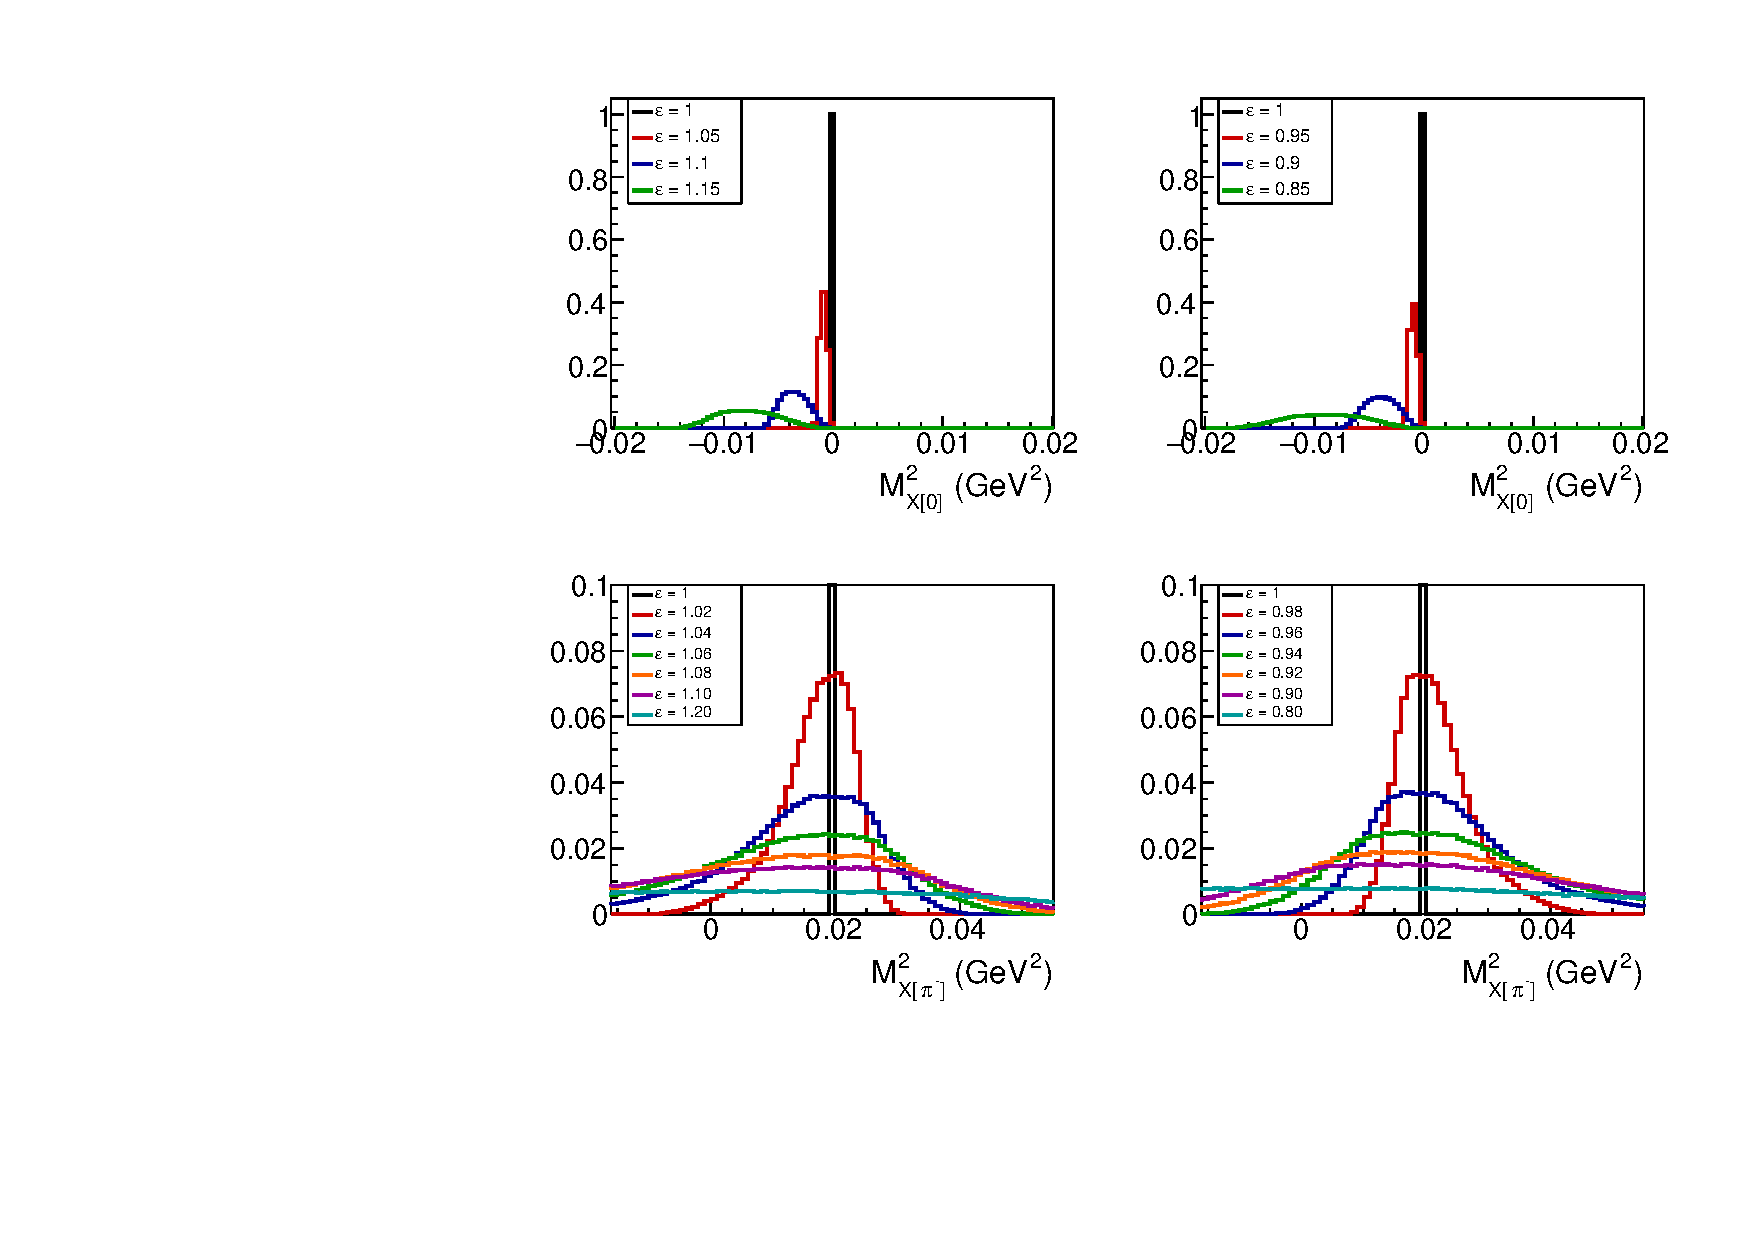
\includegraphics[width=\textwidth]{pictures/mm_pr_fsi_new2.pdf}}
\caption{\small Multi-colored histograms show the distributions of $M_{X[0]}^{2}$ (upper panels) and $M_{X[\pi^{-}]}^{2}$ (lower panels) plotted assuming that the proton momentum magnitude changes as $p'_{p'} = \varepsilon p_{p'}$ for all events in the sample. Different colors correspond to different values of $\varepsilon$. Black histograms are given as a reference and correspond to the case when no momentum alterations happen (i.e. $\varepsilon = 1$ for all events). All shown histograms contain equal numbers of events and are normalized in a way that the maximum of the $\varepsilon=1$ histogram is equal to one. The histograms that correspond to the same missing quantity have identical binning. For the quantity $M_{X[\pi^{-}]}^{2}$, shown in the lower panels, note the following, (i) the distributions are zoomed in on small $y$ and (ii) the change in $\varepsilon$ values between the magenta and cyan histograms is five times larger than for all other neighboring histograms. } \label{fig:mm_pr_fsi}
\end{center}
\end{figure}



The multi-colored histograms in Fig.~\ref{fig:mm_pip_fsi} show the distributions of $M_{X[0]}^{2}$ (upper panels) and $M_{X[\pi^{-}]}^{2}$ (lower panels) considering the $\pi^{+}$ to be the affected hadron, which means that all positive pions in the sample change their momenta as $p'_{\pi^{+}} = \varepsilon p_{\pi^{+}}$. Various histogram colors correspond to different values of $\varepsilon$, which are specified in the plots. The quantity $M_{X[0]}^{2}$ is plotted for the sizable deviations of $\varepsilon$ from unity (for $\varepsilon$ from 0.4 to 1.6 in increments of 0.2), since it turns out to be rather insensitive to the change of pion momenta. The quantity $M_{X[\pi^{-}]}^{2}$, being more sensitive to the $\pi^{+}$ momentum change, is plotted for $\varepsilon$ from 0.90 to 1.10 with 0.02 increments and also for $\varepsilon$ of 0.8 and 1.2. 



The multi-colored histograms in Fig.~\ref{fig:mm_pr_fsi} show the distributions of $M_{X[0]}^{2}$ (upper panels) and $M_{X[\pi^{-}]}^{2}$ (lower panels) considering the proton to be the affected hadron, which means~that all final protons in the sample change their momenta as $p'_{p'} = \varepsilon p_{p'}$. Various colors~correspond to different values of $\varepsilon$, which are specified in the plots. The quantity $M_{X[0]}^{2}$, being moderately sensitive to the proton momentum change, is plotted for $\varepsilon$ from 0.85 to 1.15 in increments of 0.05, while the quantity $M_{X[\pi^{-}]}^{2}$, being quite sensitive to the proton momentum change, is plotted for $\varepsilon$ from 0.90 to 1.10 with 0.02 increments and also for $\varepsilon$ of~0.8~and~1.2.  

\everypar{\looseness=-1}
The black histograms in Figs.~\ref{fig:mm_pip_fsi} and~\ref{fig:mm_pr_fsi} are given as a reference and correspond to the case when no hadron momentum alterations occur ($\varepsilon = 1$ for all events). All histograms in these figures have equal numbers of events and are normalized in a way that the maximum of the reference histogram is equal to one. The histograms that correspond to the same missing quantity have identical binning in both figures. For the quantity $M_{X[\pi^{-}]}^{2}$, note the following: (i) the distributions are zoomed in on small $y$ to demonstrate their structure and (ii) the change in $\varepsilon$ values between the magenta and cyan histograms is five times larger than for all other neighboring histograms.


\everypar{\looseness=-1}
Examination of the plots in Figs.~\ref{fig:mm_pip_fsi} and \ref{fig:mm_pr_fsi} allows for several interesting conclusions to be made. First, the quantity $M_{X[\pi^{-}]}^{2}$ turns out to be far more sensitive to hadron momentum alterations than $M_{X[0]}^{2}$. Besides this, both missing quantities turn out to be more sensitive to changes in the proton momentum than to changes in the pion momentum. Specifically, for $M_{X[\pi^{-}]}^{2}$, when the same values of $\varepsilon$ are considered for both types of affected hadrons, the distributions plotted for the case of affected protons are about three times lower in height and correspondingly significantly larger in spread than their analogues for the case of affected pions\footnote[8]{Note that as the $\varepsilon\!=\!1$ histogram is always one bin wide, the global normalization of the colored~histograms is bin width specific. The relation of the latter to each other is meanwhile stable, and hence informative.}. 



%\everypar{\looseness=-1}
In addition to that, the quantity $M_{X[\pi^{-}]}^{2}$ demonstrates a very peculiar feature: being plotted for the same set of $\varepsilon$ values, the $M_{X[\pi^{-}]}^{2}$ distributions form absolutely different patterns for the two types of affected hadrons. Specifically, when the $\pi^{+}$ is affected, the distributions demonstrate a clear one-sided agglomeration with respect to the position of $m_{\pi^{-}}^{2}$, which is left-sided for $\varepsilon > 1$ and right-sided for $\varepsilon < 1$. Meanwhile, when the proton is the affected hadron, the distributions are widely spread at both sides of $m_{\pi^{-}}^{2}$ for both cases of $\varepsilon > 1$ and $\varepsilon < 1$. 


\everypar{\looseness=-1}
This effect can be understood upon closer examination of the final expression in Eq.~\eqref{eq:mm_pim_fsi}. If $\varepsilon > 1$, the quantity in the curly brackets is positive for all events at the right of $m_{\pi^{-}}^{2}$. Meanwhile, if $\varepsilon < 1$, this quantity is negative for almost all events at the left of $m_{\pi^{-}}^{2}$. This general disposition is valid for both types of affected hadrons. However, the interrelation between the momentum and energy terms in the curly brackets turns out to differ for pions and protons. Specifically, for the same values of $\overrightarrow{p}_{\!h}$ for the cases of $h=\pi^{+}$ and $h=p'$, the values of the momentum term are identical, while the absolute value of the energy term for protons is systematically lower than for pions due to the larger mass of the former. As a result, the distributions plotted for the case of affected protons contain more events at the right of $m_{\pi^{-}}^{2}$ for $\varepsilon>1$ (and vice versa, at the left of $m_{\pi^{-}}^{2}$ for $\varepsilon<1$), if compared to the case of pion momentum alterations.


It is also noteworthy that for small values of $p_{h}$, the quantity $(E'_{h}~-~E_{h})$ in Eq.~\eqref{eq:mm_pim_fsi} gives almost indistinguishable results for $h=\pi^{+}$ and $h=p'$. However, the mismatch builds up with the momentum increase. This is due to the fact that for low-momentum hadrons the non-relativistic approximation is applicable, which suppresses the dependence of the considered quantity on the hadron mass. This means that events at the right of $m_{\pi^{-}}^{2}$ for $\varepsilon > 1$ (as well as at the left of $m_{\pi^{-}}^{2}$ for $\varepsilon < 1$) mainly correspond to non-relativistic affected hadrons. Meanwhile, in the considered event sample, protons are mostly non-relativistic, while the majority of pions is relativistic, which reflects the observed difference in the population of the aforementioned areas in the $M_{X[\pi^{-}]}^{2}$ distributions.



Also note that the $M_{X[\pi^{-}]}^{2}$ distributions that correspond to symmetric deviations of $\varepsilon$ from unity, although visually mostly looking as symmetric reflections of each other, have nevertheless asymmetric event allocation. The asymmetry mainly originates from the contribution of the second term in the final expression of Eq.~\eqref{eq:mm_pim_fsi}, which, being always negative, tosses extra events to the left of $m_{\pi^{-}}^{2}$ for all $\varepsilon$ values. As the deviation of $\varepsilon$ from unity grows, the asymmetry grows as well, being accompanied by the gradual shift of the distribution maxima to the left for both options of $\varepsilon > 1$ and $\varepsilon < 1$. The intensity of this effect differs for the two types of affected hadrons: for the case of $h=\pi^{+}$, the effect is truly insignificant for all considered here $\varepsilon$ values, while for $h=p'$ the asymmetry in the event allocation becomes noticeable for deviations of $\varepsilon$ from unity of more than $\sim$~10\%.



With the sensitivity of the missing quantities to hadron momentum alterations now better understood, one can turn to the case when the value of $\varepsilon$ can vary in a certain range among events in the event sample, for example, in the range from 0.8 to 1.2 in increments of 0.01, which results in 41 $\varepsilon$ values in total. The portion of events that carry each value of $\varepsilon$ is then determined by the probability density function $\xi(\varepsilon)$. 


Below the shape of the missing quantities is examined, assuming different types of the probability density function $\xi(\varepsilon)$. As the quantity $M_{X[0]}^{2}$ was found to have little sensitivity to changes in the hadron momentum, only the quantity $M_{X[\pi^{-}]}^{2}$ will be further illustrated with the two types of affected hadrons (proton and positive pion) separately considered.


In this study, the following four probability density functions $\xi(\varepsilon)$ are tested: uniform, linear, quadratic, and cubic. The corresponding distributions of the quantity $\xi(\varepsilon)\Delta\varepsilon$ are shown in Fig.~\ref{fig:density}, where $\Delta\varepsilon=0.01$ is the increment of the considered $\varepsilon$ values. Each $\xi(\varepsilon)$ is normalized to unity. The values on the $y$-axis reflect the portion of events in the sample that correspond to a particular value of $\varepsilon$. For simplicity, all tested here probability density functions are taken to be symmetric with respect to $\varepsilon=1$, which assumes equal portions of events with the same percentage of the momentum gain and loss to be present in the sample.

The uniform probability density function corresponds to the black histogram on the left panel of Fig.~\ref{fig:density} and represents the case when equal event portions carry various values of $\varepsilon$. In this example, each of 41 considered $\varepsilon$ values acquires a portion of about 2\% of events in the sample. The uniform probability density function, although hardly being physical, gives the advantage of impartial non-weighted judging of isolated contributions of events with different values (or subranges) of $\varepsilon$ to the resulting distributions of the missing quantities.


\begin{figure}[htp]
\begin{center}
\framebox{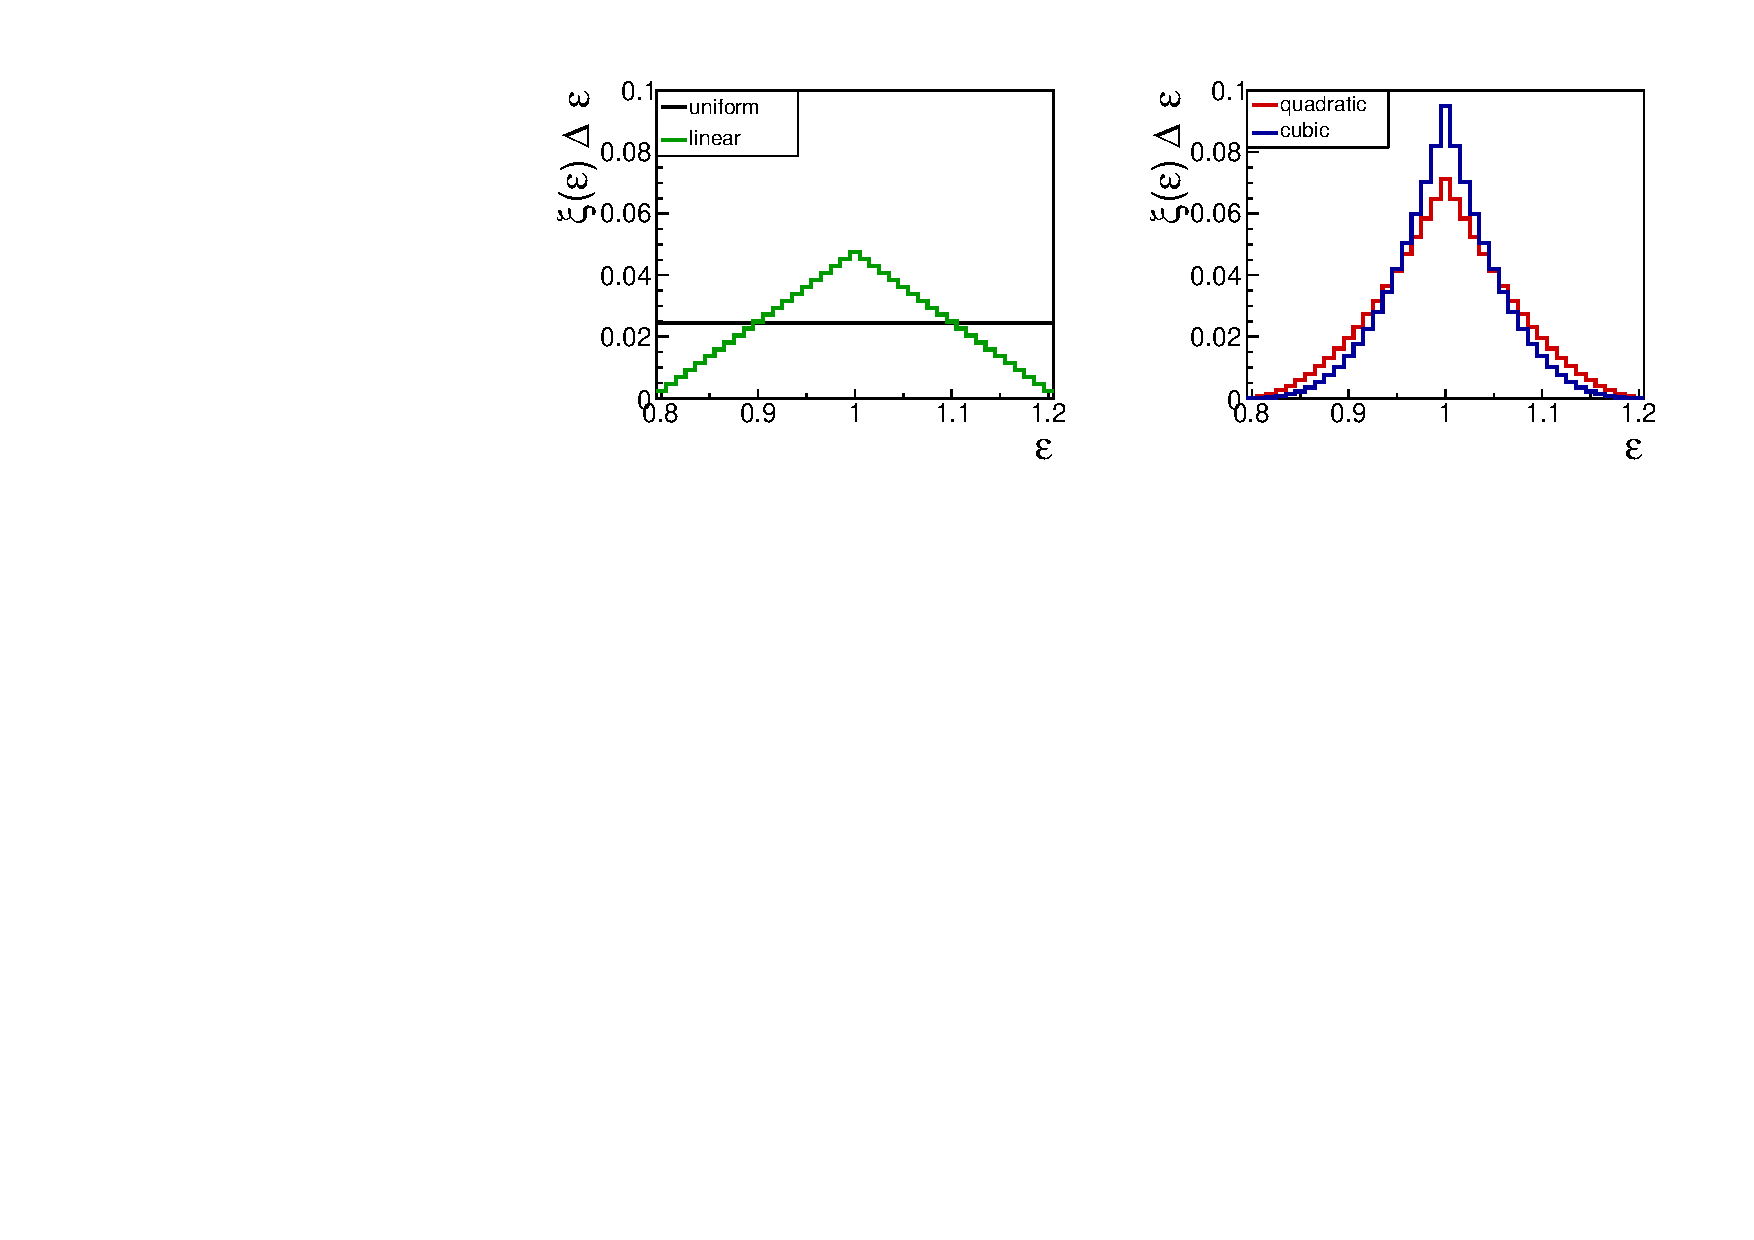
\includegraphics[width=\textwidth]{pictures/density.pdf}}
\caption{\small Distributions of the quantity $\xi(\varepsilon)\Delta\varepsilon$ for four types of the probability density functions $\xi(\varepsilon)$ considered in this study, i.e. uniform (black), linear (green), quadratic (red), and cubic (blue). The value of $\varepsilon$, which represents the degree of hadron momentum alterations, is assumed to vary in the range from 0.8 to 1.2 in increments of $\Delta\varepsilon=0.01$. Each  $\xi(\varepsilon)$ is normalized to unity. The values on the $y$-axis reflect the portion of events in the sample that carry a particular value of $\varepsilon$.  } \label{fig:density}
\end{center}
\end{figure}
\begin{figure}[htp]
\begin{center}
\framebox{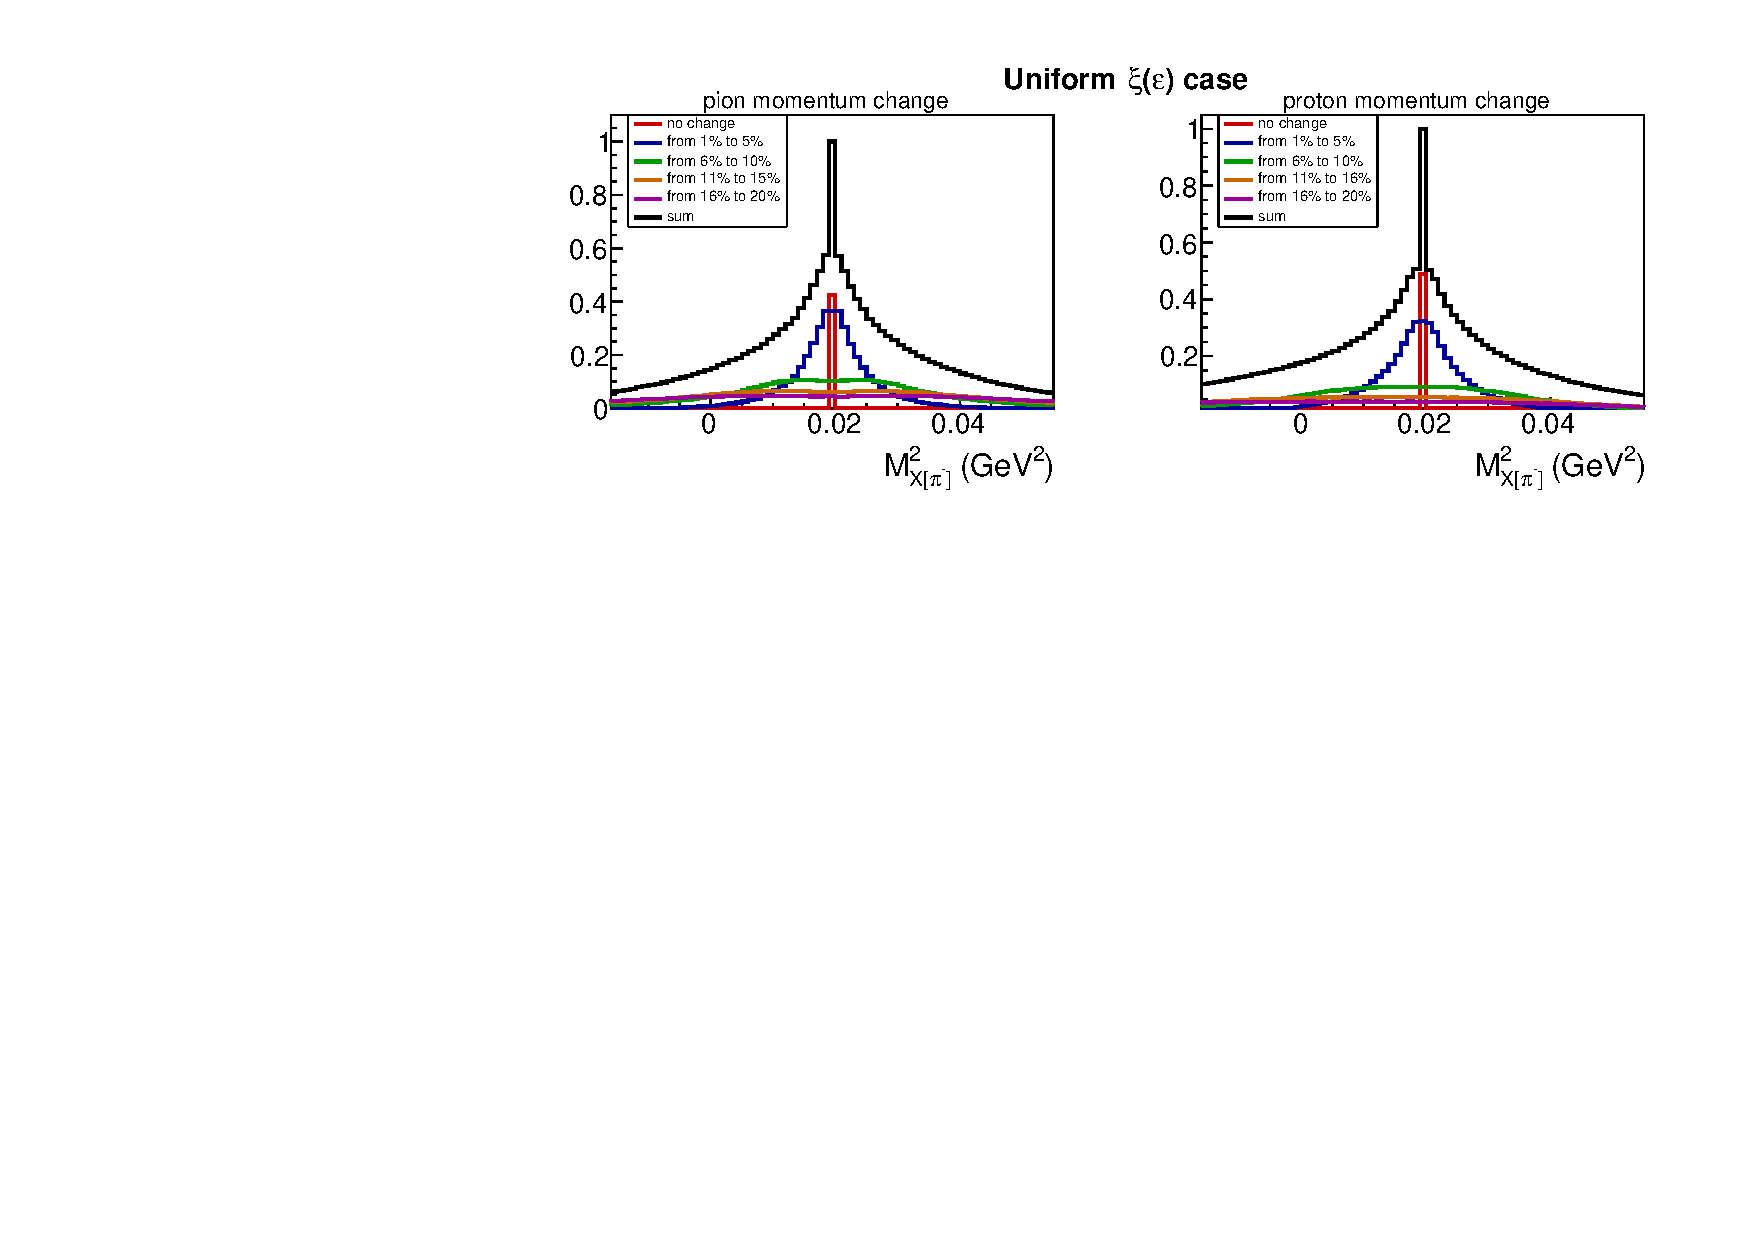
\includegraphics[width=\textwidth]{pictures/mm_fsi_detail_new.pdf}}
\caption{\small Distributions of $M_{X[\pi^{-}]}^{2}$ considering the uniform distribution of $\varepsilon$ values for two types of affected final hadrons, i.e. the positive pion (left) and the proton (right). The multi-colored histograms show the contributions from different subranges of $\varepsilon$ (specified in the plots), while the black histogram shows their sum. Note that the red histogram corresponds to a single value of $\varepsilon = 1$, while each other colored histogram incorporates ten values of $\varepsilon$, which means that the red histogram contains ten times less events than each other colored histogram.} \label{fig:mm_fsi_detail}
\end{center}
\end{figure}
\newpage

Figure~\ref{fig:mm_fsi_detail} shows the distributions of $M_{X[\pi^{-}]}^{2}$ considering a uniform distribution of $\varepsilon$ values for two types of affected hadrons, i.e. the positive pion (left) and the proton (right). The multi-colored histograms show the contributions from different subranges of $\varepsilon$, while the black histogram shows their sum. Note that the red histogram, which corresponds to the absence of momentum alterations, includes just one value of $\varepsilon = 1$, while each other colored histogram incorporates ten values of $\varepsilon$. Assuming the uniform $\xi(\varepsilon)$, this means that the red histogram contains ten times less events than each other colored histogram. 


As seen in Fig.~\ref{fig:mm_fsi_detail}, events with small momentum alterations ($\lesssim$ 5\%), although acquiring considerable smearing, still form a distinct peak at the position of $m_{\pi^{-}}^{2}$. However, events with larger momentum alterations ($\gtrsim$ 5\%) lose their peaked structure and tend to form a flat background, which resembles the background observed in experimental distributions of $M_{X[\pi^{-}]}^{2}$ for the reaction occurring off a proton bound in a deuteron~\cite{Skorodumina:2015rea,skorodum_an_note:2019}.

In Fig.~\ref{fig:mm_fsi_detail} one more interesting feature can be observed. Specifically, for the proton momentum alterations (right panel), the left tail of the total distribution (black histogram) contains noticeably more events than its right tail, whereas for the $\pi^{+}$ momentum alterations, both tails look equally populated (left panel). This effect originates from the described above asymmetry in the allocation of events that correspond to symmetric deviations of $\varepsilon$~from~unity, which is more pronounced for the case of affected protons.

%\afterpage{\clearpage}




%\afterpage{\clearpage}
\begin{figure}[!ht]
\begin{center}
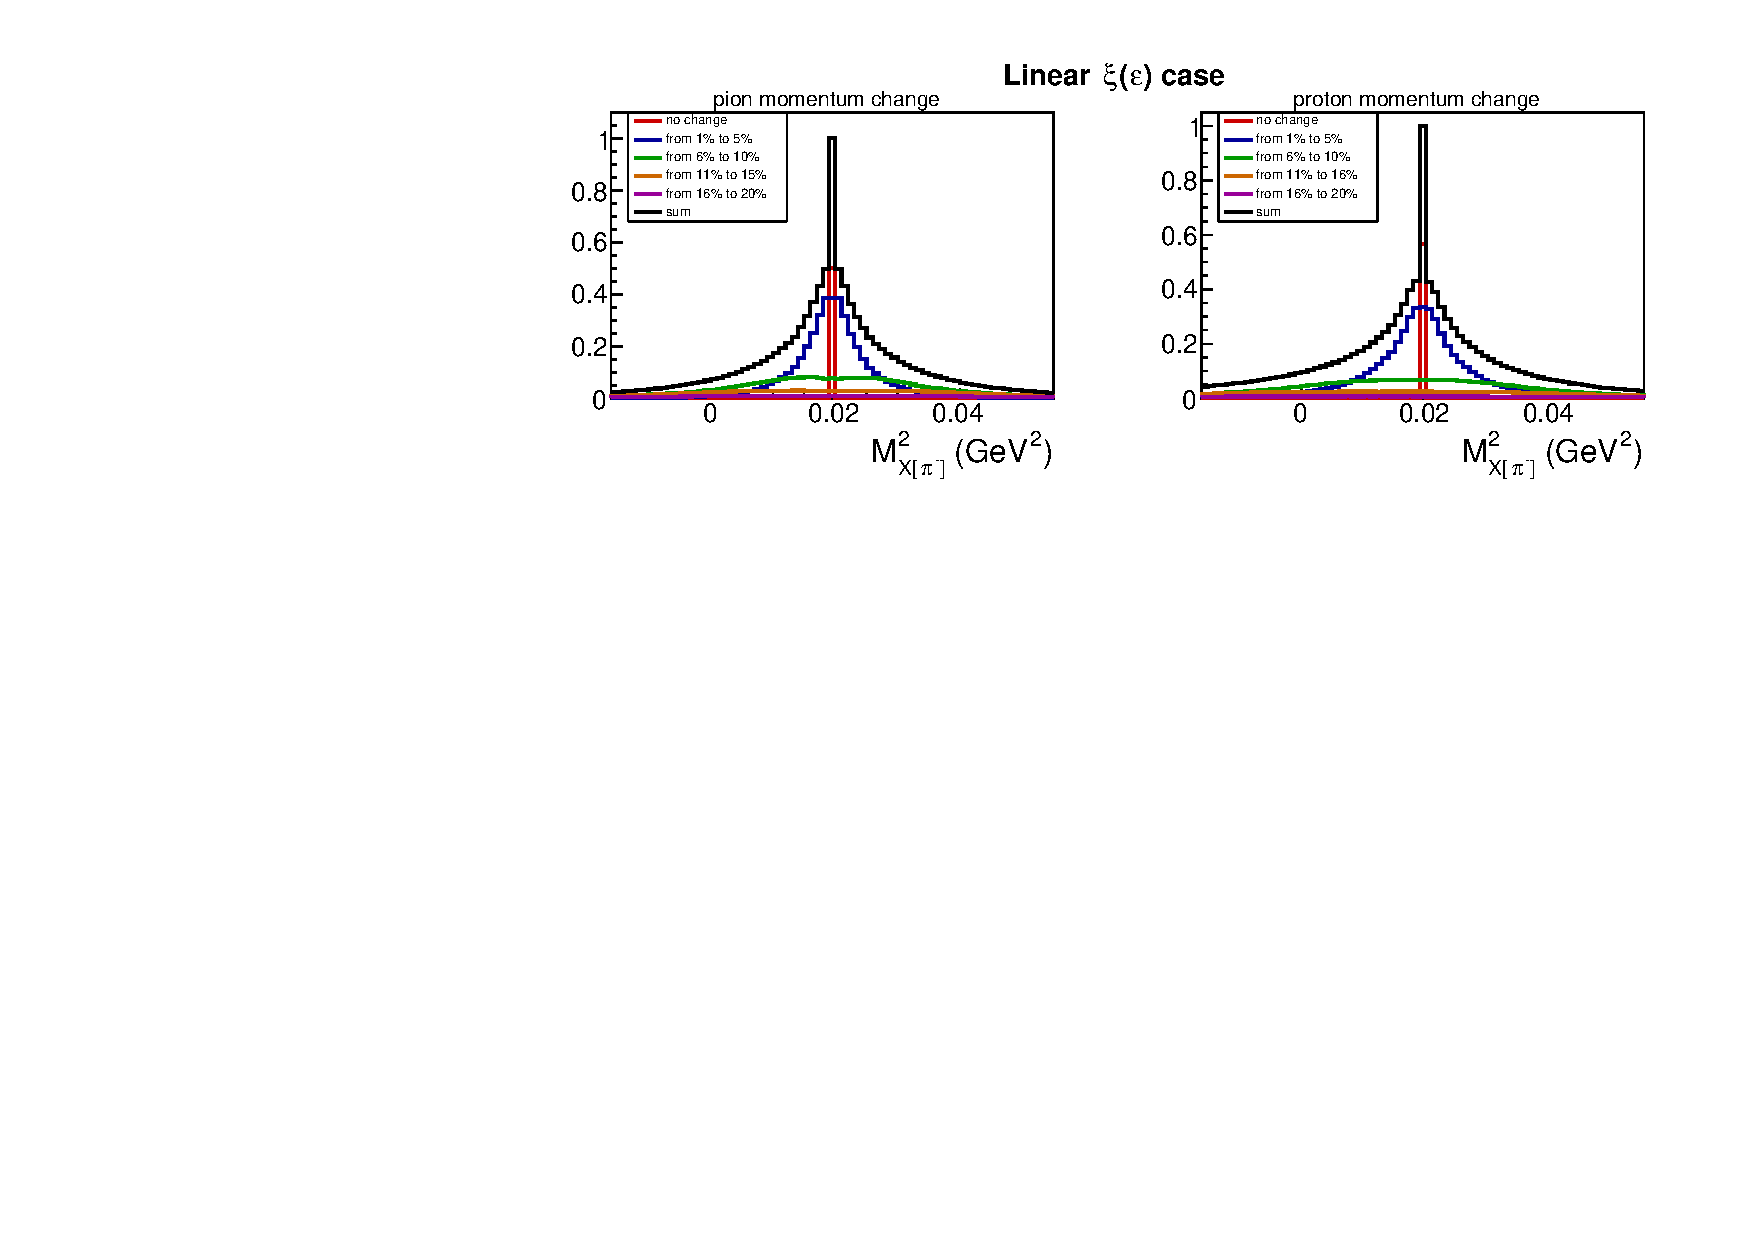
\includegraphics[width=\textwidth]{pictures/mm_fsi_detail_linear_new.pdf}
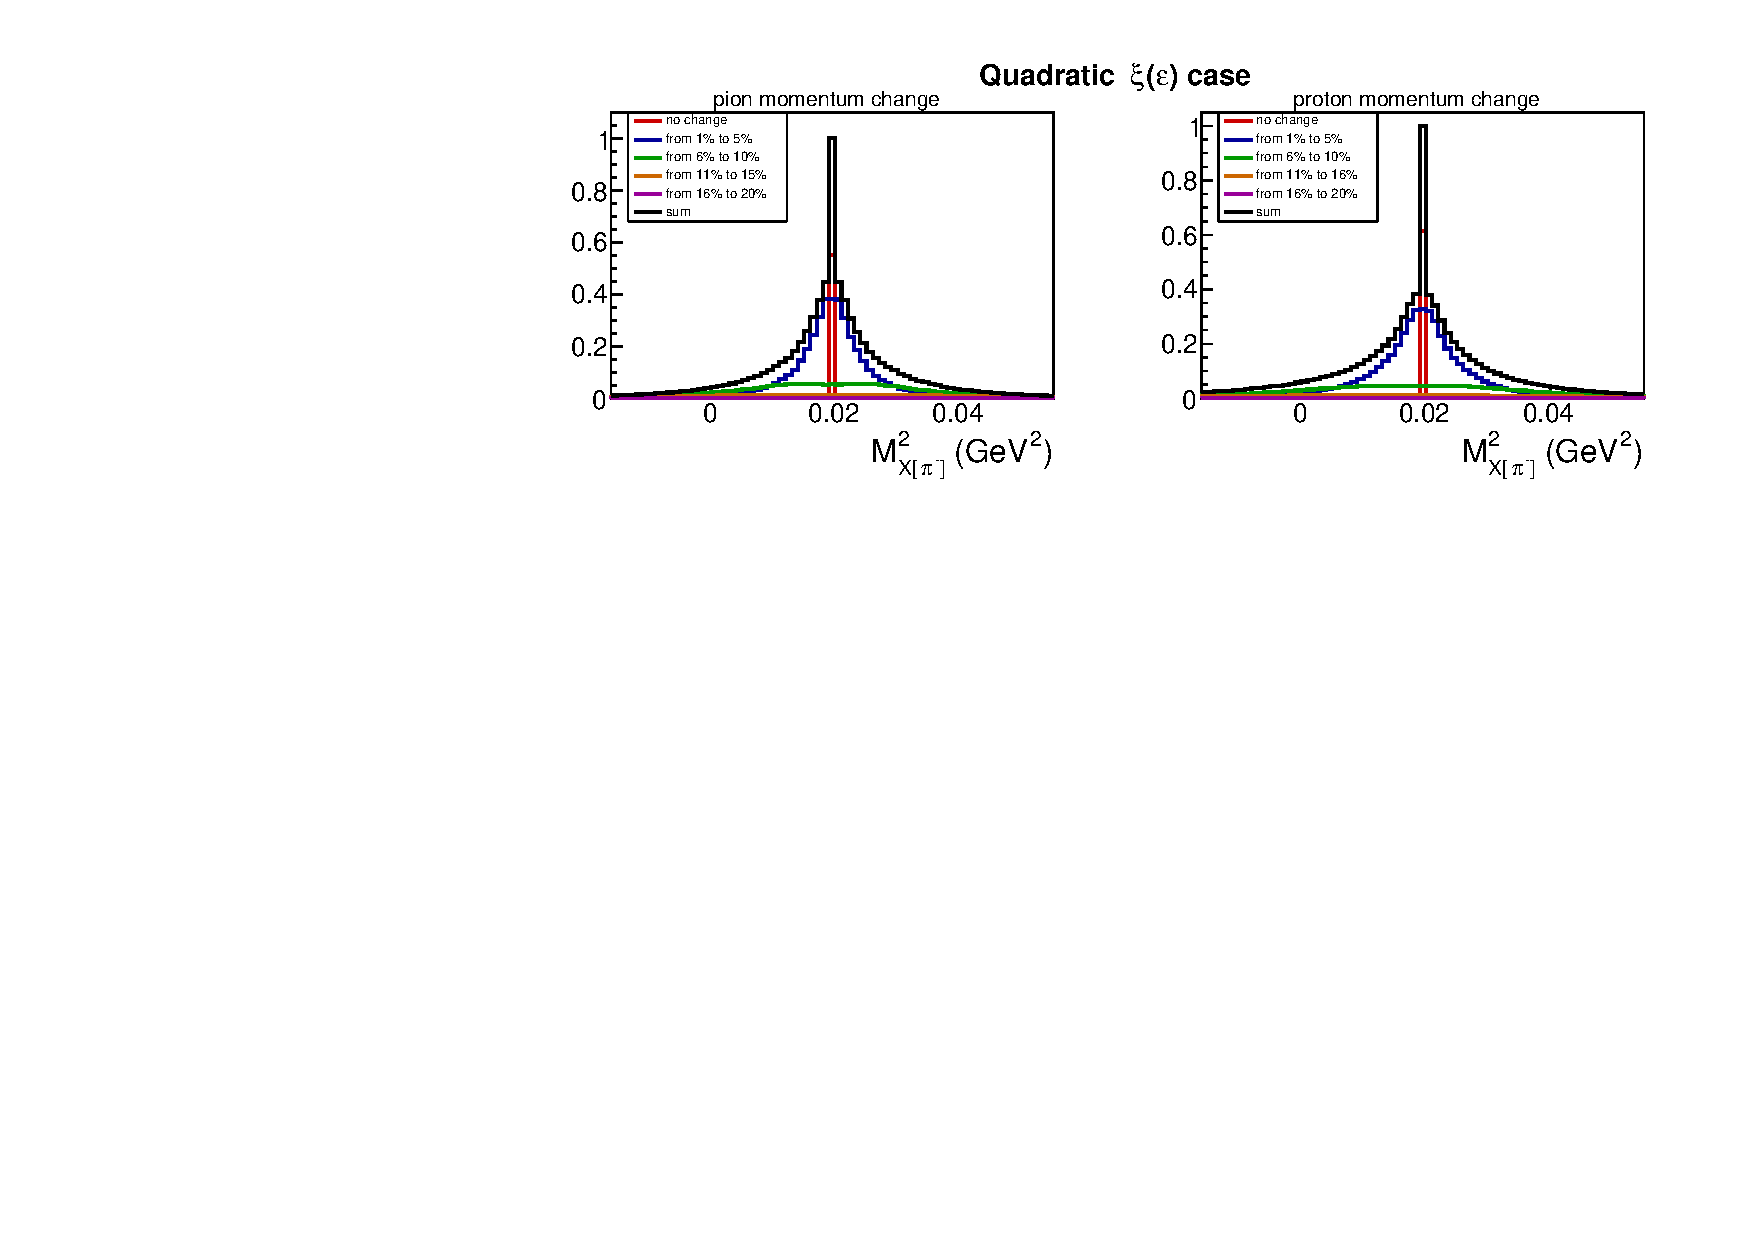
\includegraphics[width=\textwidth]{pictures/mm_fsi_detail_sq_new.pdf}
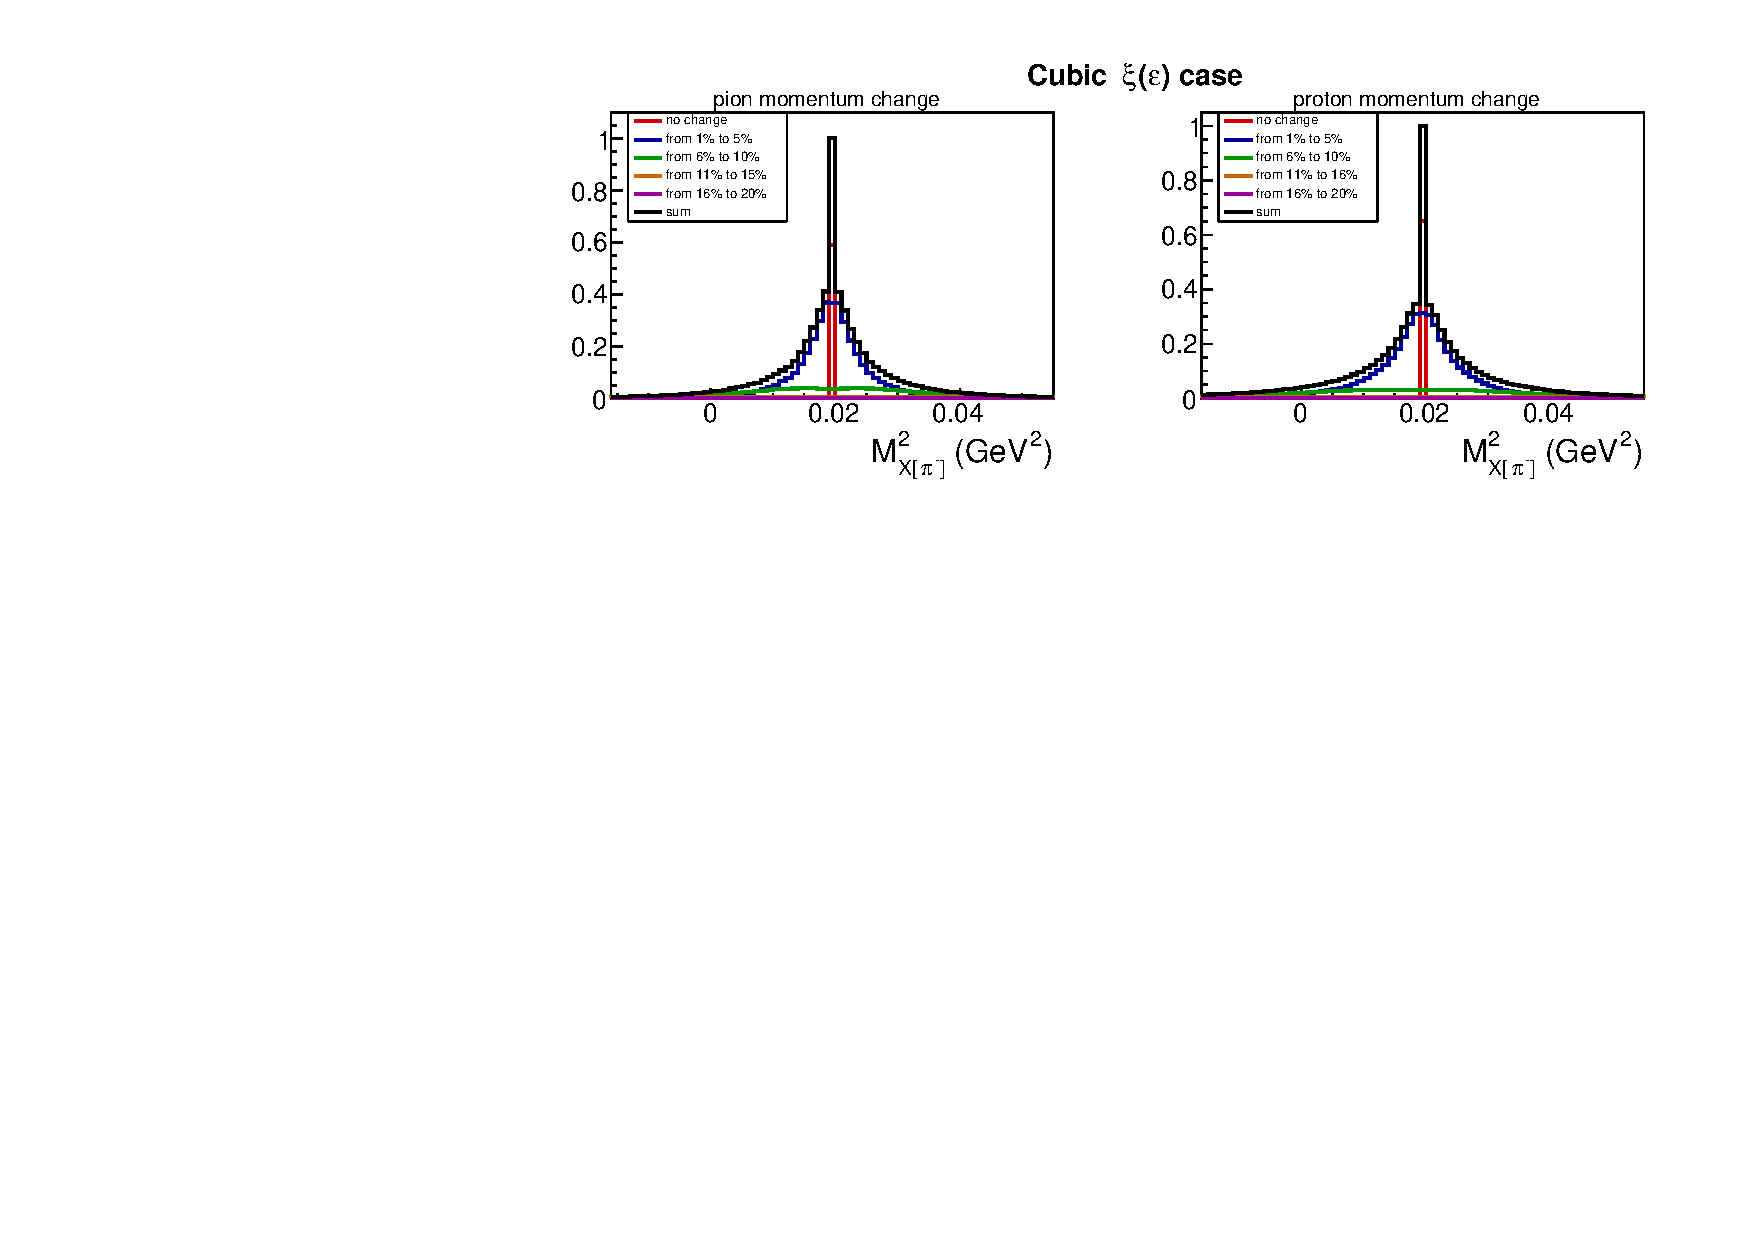
\includegraphics[width=\textwidth]{pictures/mm_fsi_detail_cube_new.pdf}
\end{center}
\vspace{-0.6cm}
\caption{\small Distributions of $M_{X[\pi^{-}]}^{2}$ considering the non-uniform distributions of $\varepsilon$ values for two types of affected final hadrons, i.e. the positive pion (left) and the proton (right). The cases of linear, quadratic, and cubic probability density functions are shown from top to bottom. The multi-colored histograms show the contributions from different subranges of $\varepsilon$ (specified in the plots), while the black histogram shows their sum. }
\label{fig:fsi_combined}
\end{figure}

Now one can employ three non-uniform probability density functions: linear, quadratic, and cubic, which correspond to the green, red, and blue curves in Fig.~\ref{fig:density}, respectively. All of them imply the gradual probability decline with growing momentum deviations, letting events with no momentum alterations to form the largest portion in the sample. Meanwhile, the size of the unaffected event portion and the degree of the probability decline are different for each function.


Figure~\ref{fig:fsi_combined} shows the distributions of $M_{X[\pi^{-}]}^{2}$ plotted employing the aforementioned non-uniform density functions $\xi(\varepsilon)$ for the two types of affected hadrons, i.e. the positive pion (left) and the proton (right). The cases of linear, quadratic, and cubic probability density functions are shown from top to bottom. Again, the multi-colored histograms show the contributions from different subranges of $\varepsilon$, while the black histogram shows their sum.

From Fig.~\ref{fig:fsi_combined} one can conclude that for a probability density function that peaks at $\varepsilon = 1$ and gradually declines with growing degree of momentum alterations, the cumulative contribution from large momentum alterations ($\gtrsim$~10~\%) to the total distribution thins to imperceptible values. The disturbances of the resulting distributions then do not form substantial flat background, staying on a level of smearing.


\afterpage{\clearpage}






